\PassOptionsToPackage{dvipsnames,table}{xcolor}
\documentclass[10pt]{beamer}
\usetheme[options]{Madrid} 
\usepackage{../../latex/Cours}

\begin{document}
	
	\input{\detokenize{../../latex/MacrosCours.tex}}
\setcounter{numchap}{15}
\pythonmode
\newcommand{\KNN}{\cnum Algorithme des $k$ plus proches voisins}

% Complément à 2
\begin{frame}
	\mframe{\KNN}
	\begin{alertblock}{Principe de l'algorithme}
		\begin{itemize}
			\item<1-> L'algorithme de \textcolor{red}{$k$ plus proches voisins} est un algorithme de classification des données. 
			\item<2-> On dispose d'un jeu de données qui associe chaque donnée à une classe.
			\item<3-> L'algorithme attribut à une nouvelle donnée $d$ non classée la classe majoritaire de ses $k$ plus proches voisins.
		\end{itemize}
	\end{alertblock}
\end{frame}

\begin{frame}
	\mframe{\KNN}
	\begin{exampleblock}{Exemple}
		\begin{center}
		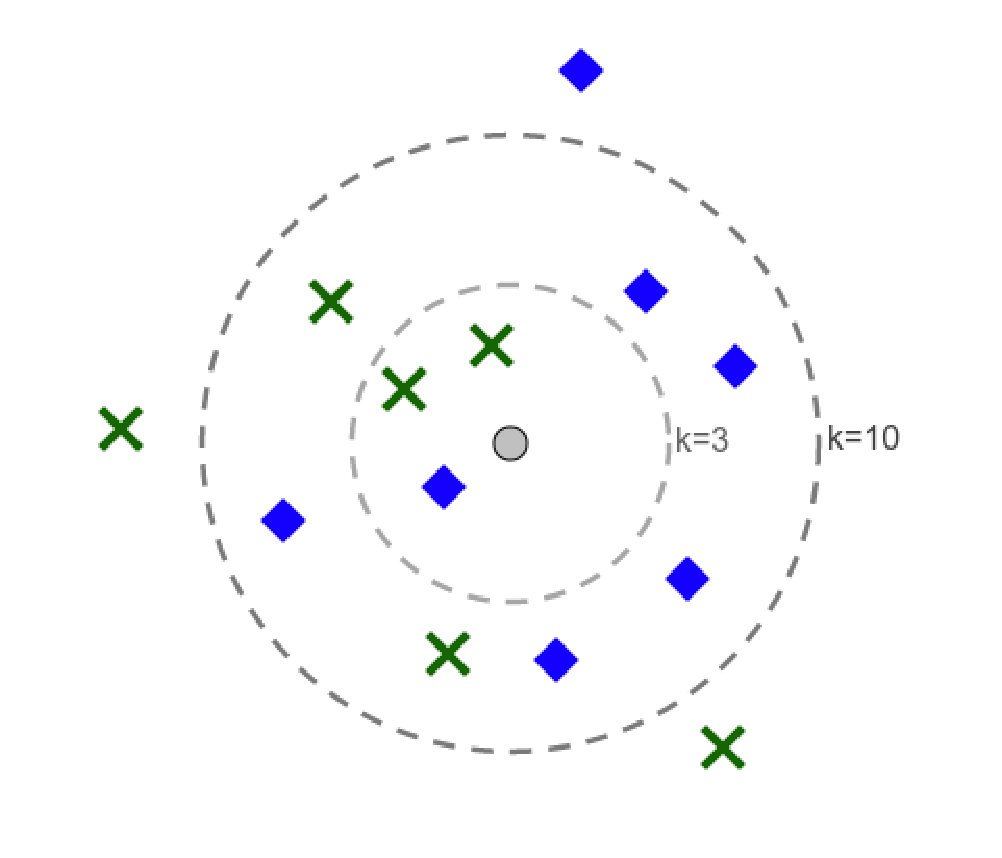
\includegraphics[scale=0.25]{knn1.eps}
		\end{center}
		Le point gris central est la donnée à classer. Quel sera le résultat de l'algorithme :
		\begin{itemize}
			\item<2-> Pour $k=3$ ?
			\onslide<3->{\textcolor{OliveGreen}{Il y 2 croix et un losange dans les 3 plus prochains voisins, la classe majoritaire est donc la croix et l'algorithme classe la donnée comme une croix.}}
			\item<4-> Pour $k=10$ ?
			\onslide<5->{\textcolor{OliveGreen}}{\textcolor{OliveGreen}{Cette fois il y a 6 losanges et 4 croix parmi les 10 plus proches voisins, la donnée est donc classée parmi les losanges.}}
		\end{itemize}
	\end{exampleblock}
\end{frame}


\begin{frame}
		\mframe{\KNN}
		\begin{block}{Remarques}
			\begin{itemize}
				\item<1-> Sur l'exemple précédent, on a utilisé la distance euclidienne dans le plan. D'autres distances sont envisageables.
				\item<2-> Le nombre de $k$ de voisins considéré influence la prédiction de l'algorithme (voir exemple précédent)
			\end{itemize}
		\end{block}
\end{frame}
\end{document}
